%==============================================================================
% Sjabloon poster bachproef
%==============================================================================
% Gebaseerd op document class `a0poster' door Gerlinde Kettl en Matthias Weiser
% Aangepast voor gebruik aan HOGENT door Jens Buysse en Bert Van Vreckem

\documentclass[a0,portrait]{hogent-poster}

\usepackage{multicol}
\usepackage{tikz}
\usetikzlibrary{positioning, shapes.geometric, calc}
\usepackage{array}


% Info over de opleiding
\course{Bachelorproef}
\studyprogramme{toegepaste informatica}
\academicyear{2025-2026}
\institution{Hogeschool Gent, Valentin Vaerwyckweg 1, 9000 Gent}

% Info over de bachelorproef
\title{Ontwikkelen van een geautomatiseerde end-to-end testworkflow om continu de productkwaliteit te meten bij talentguide.}
\author{Edis Hurtic}
\email{edis.hurtic@student.hogent.be}
\supervisor{Martine Van Audenrode}
\cosupervisor{Maryna Soufi (Talentguide BV)}

% Indien ingevuld, wordt deze informatie toegevoegd aan het einde van de
% abstract. Zet in commentaar als je dit niet wilt.
\specialisation{Full stack developer}
\keywords{Testing AI workflow, kwaliteitsborging, HR tooling, geautomatiseerde testomgeving}
\projectrepo{https://github.com/HeyEdis/edis-hurtic-hogent-bachproef}

\newcommand{\phaseitem}[3]{%
    \noindent
    \begin{tabular}{@{}m{0.0\linewidth}@{\hspace{0.15\linewidth}}m{0.85\linewidth}@{}}
        \centering
        \raisebox{0.5cm}{%
            \begin{tikzpicture}[baseline=(icon.base)]
                \node[circle, fill=#1!18, draw=#1, line width=2.5pt, minimum size=2.9cm] (icon) {};
                \begin{scope}[scale=1.55]
                    #2
                \end{scope}
            \end{tikzpicture}%
        }
        &
        \raggedright #3
    \end{tabular}
    \par\vspace{0.0\baselineskip}
}

\newlength{\scorecardxpadding}
\newlength{\scorecardypadding}
\setlength{\scorecardxpadding}{0.6cm}
\setlength{\scorecardypadding}{0.6cm}

\newcommand{\scorecard}[4]{%
    \noindent
    \begin{tikzpicture}
        \node[
        fill=#2!10,
        rounded corners=8pt,
        inner xsep=\scorecardxpadding,
        inner ysep=\scorecardypadding,
        minimum width=\linewidth,
        text width=\dimexpr\linewidth-2\scorecardxpadding\relax,
        align=left,
        anchor=north west
        ] {%
            {\large\titlefont #1}\hfill{\large\textbf{\color{#2}#3}}
            \par\vspace{0.2\baselineskip}
            #4
        };
    \end{tikzpicture}
    \par\vspace{0.45\baselineskip}
}

\begin{document}

\maketitle

\begin{abstract}
Dit onderzoek vindt plaats in opdracht van talentguide, een organisatie die AI gedreven inzichten in competenties van arbeiders levert om talentontwikkeling en strategische personeelsplanning te bevorderen. In het bijzonder is het probleem van een lage productkwaliteit onderzocht van het SaaS-platform. Die veroorzaakt is door een gebrek aan kwaliteitsmetingen en end-to-end testen. Dit leidt tot instabiele releases naar de productieomgeving toe wat de gebruikerservaring verstoort.
De hoofdonderzoeksvraag luidt: hoe kan een geautomatiseerd end-to-end testsysteem worden opgezet dat het product continu meet, zodat kwaliteit is verankerd in het ontwikkelingsproces en ervoor zorgt dat ontwikkelaars geen kostbare tijd moeten nemen om volledig nieuwe testen te schrijven?
De gevolgde methodologie is opgedeeld in vier fasen. Eerst is een nulmeting uitgevoerd door de bestaande GitHub CI/CD pijplijn en het Sentry dashboard te analyseren om de kritieke fouten te identificeren.
In de tweede fase zijn de richtlijnen en benodigheden onderzocht hierbij zijn de richtlijnen voor de vaardigheidsbestanden zijn gedefinieerd, hoe de keten samenwerkt geïllustreerd, wat de testdekking niveaus zijn en de functionele en non-functionele technische richtlijnen voor elk vaardigheidsbestand. Dit waarborgt dat de AI output kan integreren binnen de codebase.
In de derde fase is het prototype ontwikkeld. Dit is een geautomatiseerde workflow dat op basis technische richtlijnen de AI agents aanstuurt om met minimale input van ontwikkelaars kwalitatieve end-to-end testen te generen. 
In de laatste fase is de gegenereerde testoutput geëvalueerd op uitvoerbaarheid, functionele dekking, richtlijnconformiteit en traceerbaarheid.
Er wordt verwacht dat dit prototype zal dienen als een betrouwbare testprocedure die kwaliteitsborging integreert in het ontwikkelingsproces met een minimale belasting van het ontwikkelingsteam. Deze resultaten zullen leiden tot een verhoogde betrouwbaarheid van het SaaS-platform met een toekomstgerichte aanpak.
\end{abstract}

\begin{multicols}{2} % This is how many columns your poster will be broken into, a portrait poster is generally split into 2 columns

\section{Introductie}

73,4\% van de foutmeldingen zijn pas in productie zichtbaar. Dit betekent dat een groot deel van de kwaliteitsproblemen pas verschijnen wanneer echte gebruikers met talentguide werken. Deze bachelorproef onderzoekt hoe de detectie van deze foutmeldingen naar de development omgeving verschoven kan worden, zodat de eindgebruiker niet de eerste tester is.

\section{Methodologie}

\phaseitem{hogent-blue}{
    \draw[hogent-blue, line width=2.5pt] (-0.12,0.12) circle (0.22);
    \draw[hogent-blue, line width=2.5pt] (0.05,-0.05) -- (0.45,-0.45);
}{\bigskip
    \textbf{Fase 1 - Nulmeting van de huidige staat}\\
    Analyse van GitHub CI/CD en Sentry om te bepalen waar foutmeldingen zichtbaar worden.
}

\phaseitem{hogent-ochre}{
    \draw[hogent-ochre, line width=2pt] (-0.38,-0.52) rectangle (0.38,0.52);
    \draw[hogent-ochre, line width=2pt] (-0.2,0.25) -- (0.25,0.25);
    \draw[hogent-ochre, line width=2pt] (-0.2,0) -- (0.25,0);
    \draw[hogent-ochre, line width=2pt] (-0.2,-0.25) -- (0.25,-0.25);
}{\bigskip
    \textbf{Fase 2 - Richtlijnen en benodigdheden}\\
    Vastleggen welke testdekking, Playwright-afspraken, vaardigheidsbestanden en kwaliteitscriteria nodig zijn.
}

\phaseitem{hogent-lightgreen}{
    \draw[hogent-lightgreen, line width=2.2pt] (-0.52,0.22) circle (0.16);
    \draw[hogent-lightgreen, line width=2.2pt] (0.02,0.22) circle (0.16);
    \draw[hogent-lightgreen, line width=2.2pt] (0.56,0.22) circle (0.16);
    \draw[hogent-lightgreen, line width=2.2pt] (-0.36,0.22) -- (-0.14,0.22);
    \draw[hogent-lightgreen, line width=2.2pt] (0.18,0.22) -- (0.40,0.22);
    \draw[hogent-lightgreen, line width=2.2pt] (0.02,0.06) -- (0.02,-0.28);
    \draw[hogent-lightgreen, line width=2.2pt] (-0.28,-0.28) rectangle (0.32,-0.62);
}{\bigskip
    \textbf{Fase 3 - Proof-of-concept}\\
    Opzetten van een AI-ondersteunde E2E-testworkflow met Ralph als uitvoeringsloop.
}

\phaseitem{hogent-darkgreen}{
    \draw[hogent-darkgreen, line width=3pt] (-0.45,0) -- (-0.12,-0.34) -- (0.48,0.38);
}{\bigskip
    \textbf{Fase 4 - Evaluatie}\\
    Beoordelen van de gegenereerde testoutput op uitvoerbaarheid, functionele dekking, richtlijnconformiteit en traceerbaarheid.
}

\section{End-to-end testketen}

De keten is opgebouwd uit controleerbare tussenstappen. Die als input dienen voor de volgende stap.

\begin{center}
    \refstepcounter{figure}
    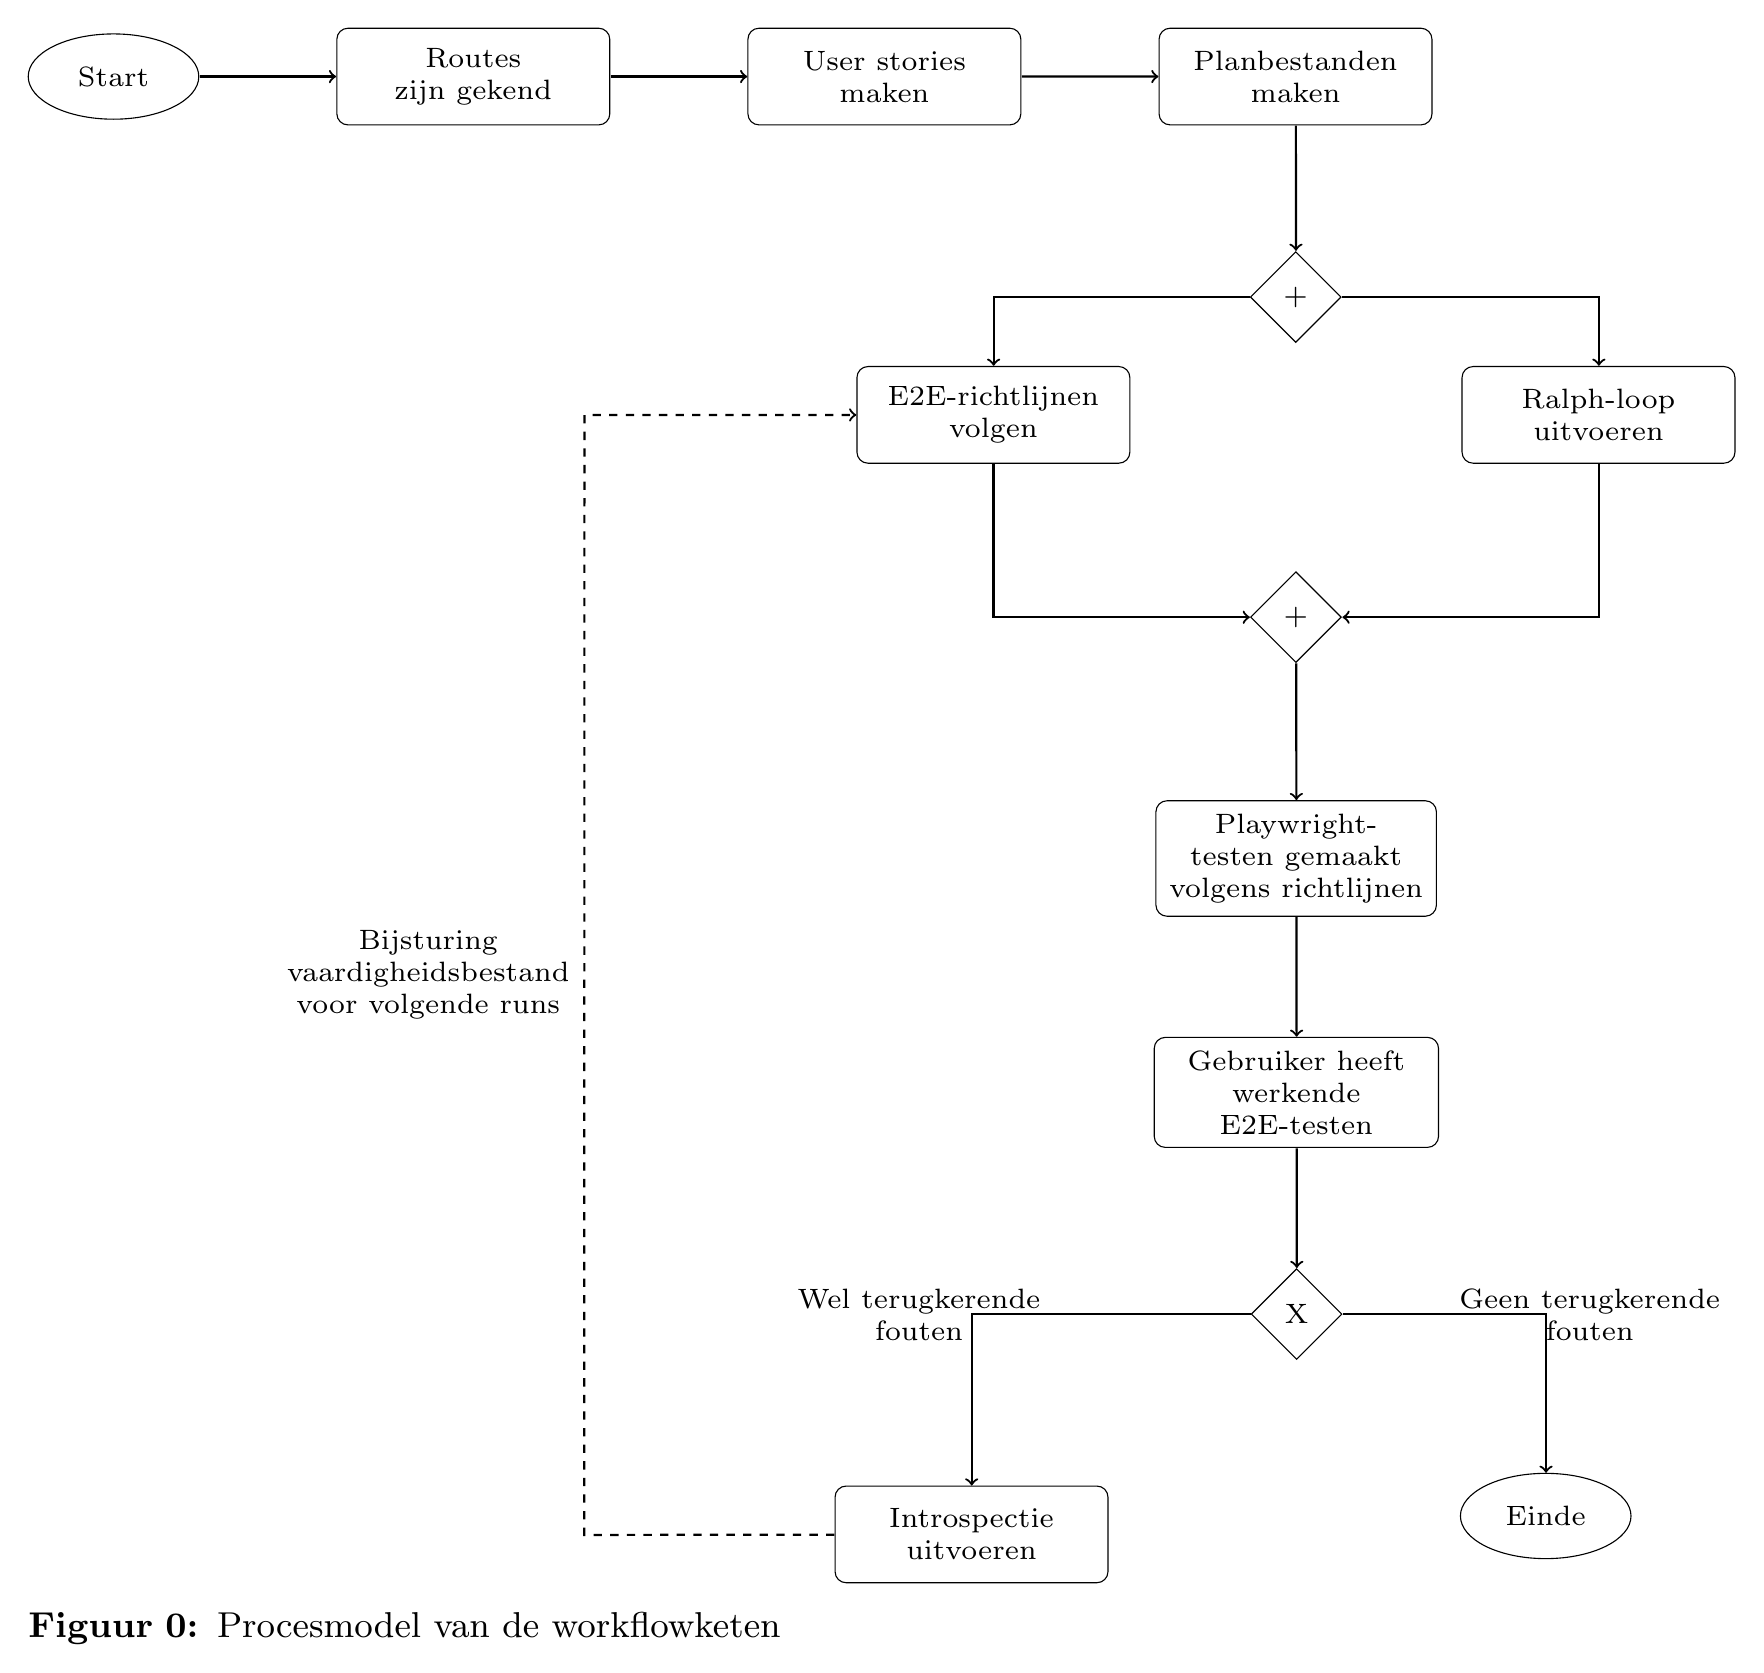
\begin{tikzpicture}[
        scale=1.44417,
        transform shape,
        node distance=1.1cm and 1.2cm,
        startend/.style={
            ellipse,
            draw,
            align=center,
            minimum width=1.5cm,
            minimum height=0.75cm,
            font=\scriptsize
        },
        activity/.style={
            rectangle,
            draw,
            rounded corners,
            align=center,
            minimum width=2.4cm,
            minimum height=0.85cm,
            font=\scriptsize
        },
        gateway/.style={
            diamond,
            draw,
            aspect=1.4,
            align=center,
            inner sep=1pt,
            minimum width=0.8cm,
            minimum height=0.8cm,
            font=\scriptsize
        },
        arrow/.style={->, thick},
        feedback/.style={->, thick, dashed}
        ]
        
        % Preparation chain
        \node[startend] (start) {Start};
        \node[activity, right=of start] (routes) {Routes\\zijn gekend};
        \node[activity, right=of routes] (stories) {User stories\\maken};
        \node[activity, right=of stories] (plans) {Planbestanden\\maken};
        
        % First AND gateway
        \node[gateway, below=1.1cm of plans] (andstart) {+};
        
        % Parallel inputs
        \node[activity, below left=0.4cm and 1.25cm of andstart] (e2e) {E2E-richtlijnen\\volgen};
        \node[activity, below right=0.4cm and 1.25cm of andstart] (ralph) {Ralph-loop\\uitvoeren};
        
        % Join gateway
        \node[gateway, below=2.0cm of andstart] (andjoin) {+};
        
        % Output
        \node[activity, below=1.20cm of andjoin] (tests) {Playwright-\\testen gemaakt\\volgens richtlijnen};
        \node[activity, minimum width=2.5cm, below=1.05cm of tests] (working) {Gebruiker heeft\\werkende\\E2E-testen};
        
        % Decision after working tests
        \node[gateway, below=1.05cm of working] (choice) {X};
        
        % End branches
        \node[activity, below left=1.3cm and 1.45cm of choice] (intro) {Introspectie\\uitvoeren};
        \node[startend, below right=1.3cm and 1.45cm of choice] (end) {Einde};
        
        % Main flow
        \draw[arrow] (start) -- (routes);
        \draw[arrow] (routes) -- (stories);
        \draw[arrow] (stories) -- (plans);
        \draw[arrow] (plans) -- (andstart);
        
        \draw[arrow] (andstart) -| (e2e);
        \draw[arrow] (andstart) -| (ralph);
        
        \draw[arrow] (e2e.south) |- (andjoin);
        \draw[arrow] (ralph.south) |- (andjoin);
        
        \draw[arrow] (andjoin) -- (tests);
        \draw[arrow] (tests) -- (working);
        \draw[arrow] (working) -- (choice);
        
        \draw[arrow] (choice) -| node[pos=0.35, left, font=\scriptsize, align=center] {Wel terugkerende\\fouten} (intro);
        \draw[arrow] (choice) -| node[pos=0.25, right, font=\scriptsize, align=center] {Geen terugkerende\\fouten} (end);
        
        % Feedback loop
        \coordinate (feedbackleft) at ($(intro.west)+(-2.2,0)$);
        \coordinate (feedbacktop) at (feedbackleft |- e2e.west);
        
        \draw[feedback] (intro.west) -- (feedbackleft)
        -- node[midway, left, font=\scriptsize, align=center] {Bijsturing\\vaardigheidsbestand\\voor volgende runs}
        (feedbacktop) -- (e2e.west);
        
        \node[
        anchor=north west,
        font=\small,
        inner sep=0pt,
        text width=\linewidth,
        align=left
        ] at ($(current bounding box.south west)+(0,-0.25)$)
        {\small\textbf{Figuur~\thefigure:} Procesmodel van de workflowketen};
        
    \end{tikzpicture}
\end{center}

\section{Resultaten en conclusie}

De AI-ondersteunde E2E-testworkflow leverde bruikbare Playwright-testoutput op voor drie geselecteerde routes. De kwaliteit werd bepaald door traceerbaarheid en minimumcriteria.
\\

\scorecard{evaluation-wizard}{hogent-darkgreen}{95\% - Excellent}{
    Sterke functionele dekking, richtlijnconformiteit en traceerbaarheid.
}

\scorecard{people}{hogent-blue}{89\% - Acceptable}{
    Hoge score, maar geen doorlopende happy-flowtest. Hierdoor daalde het kwaliteitsniveau van \textbf{Good} naar \textbf{Acceptable}.
}

\scorecard{coach-settings}{hogent-blue}{64\% - Acceptable}{
    Bruikbare testcode, maar het kwaliteitsniveau bleef \textbf{Acceptable} omdat plan- en progressartefacten ontbraken.
}

De workflow neemt het werk van ontwikkelaars niet volledig over. De ontwikkelaar blijft nodig om de scope te controleren, user stories en plannen na te kijken, gegenereerde code te reviewen en de output in de codebase te integreren. De winst zit in dat er niet vanaf nul moet begonnen worden. Hierdoor kan met minimale ontwikkelaars input e2e testen gegenereerd worden. Die ervoor zorgen dat gebruikersflows in de development omgeving eerst getest worden voordat de eindgebruiker die kan doorlopen. Dit kan direct leiden dat het foutenpercentage van 73,4\% in productie daalt.

\section{Toekomstig onderzoek}

\textbf{Meer routes evalueren}\\
De huidige evaluatie is beperkt tot drie routes. Extra routes kunnen aantonen of de workflow ook bruikbaar blijft bij andere rollen, datavormen en gebruikersflows binnen talentguide.
\bigskip
\\
\textbf{Evaluatie terugkoppelen naar Ralph}\\
In een volgende versie kan evaluatie-output opnieuw als input dienen voor de Ralph-loop. Zodat de ontwikkelaars input en tijd verminderd wordt en de workflow zichzelf volledig bijstuurd.

\end{multicols}
\end{document}
